Trong mô hình khách hàng - nhà cung cấp, nếu nhà cung cấp có thể thay đổi linh hoạt không đảm bảo đáp ứng nhu cầu của khách hàng thì khách hàng cần có giải pháp xử lí. Mô hình chống đổ vỡ (Anti Corruption Layer) là một mối quan hệ trong đó bối cảnh bị giới hạn hạ lưu sử dụng một lớp để dịch giữa ngôn ngữ của nó và ngôn ngữ của bối cảnh bị giới hạn thượng nguồn.

Trong mô hình chống đổ vỡ, mỗi bối cảnh bị giới hạn có mô hình riêng biệt và lớp chống đổ vỡ cần kiến thức về mô hình hạ lưu và thượng nguồn để bảo vệ hạ lưu và duy trì tính toàn vẹn.

%@ Façade

%@ Adapter

Trong mô hình chống đổ vỡ bối cảnh bị giới hạn hạ lưu được ký hiệu là ACL.

% Vẽ lại bản đồ tiếng Việt

% Vẽ lại bản đồ tiếng Việt

% Vẽ lại bản đồ tiếng Việt

% Vẽ lại bản đồ tiếng Việt

% Vẽ lại bản đồ tiếng Việt

% Vẽ lại bản đồ tiếng Việt

% Vẽ lại bản đồ tiếng Việt

% Vẽ lại bản đồ tiếng Việt

% Từ bản đồ lấy vi dụ cho các mô hình

% Từ bản đồ lấy vi dụ cho các mô hình

% Từ bản đồ lấy vi dụ cho các mô hình

% Từ bản đồ lấy vi dụ cho các mô hình

% Từ bản đồ lấy vi dụ cho các mô hình

% Từ bản đồ lấy vi dụ cho các mô hình

% Từ bản đồ lấy vi dụ cho các mô hình

% Từ bản đồ lấy vi dụ cho các mô hình

% Từ bản đồ lấy vi dụ cho các mô hình

% Từ bản đồ lấy vi dụ cho các mô hình

\begin{example} Trong miền vấn đề ngân hàng, thẻ tín dụng và khoản vay mua nhà không có mối quan hệ.

\begin{figure}[H]

\centering

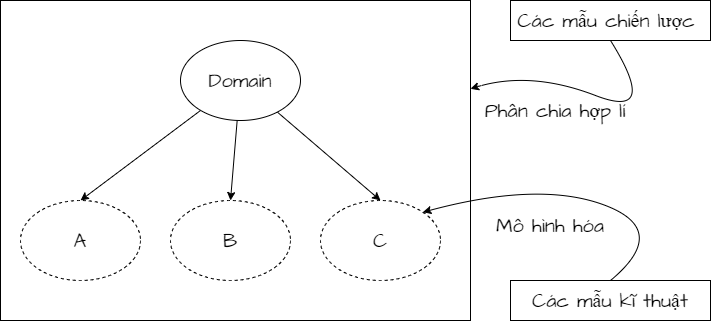
\includegraphics[scale = 0.5]{pictures/mo_hinh_rieng_biet_separate_ways/main.drawio.png}

\caption{Ví dụ mô hình riêng biệt (Separate Ways)}

\end{figure}

\end{example}

